%% !TeX program = xelatex
%\documentclass[A5,17pt,UzkyOkraj,CislaStr,StylVet,openright]{velke}

% Zakomentuj pro velké písmo
\documentclass[a4paper,11pt,twoside]{article}
\usepackage{palatino}
\usepackage{newtxmath}
\usepackage[T1]{fontenc}


\usepackage{bbold}						%% Písma
\usepackage{microtype}					%% Lepší mezery
\usepackage[utf8]{inputenc}	            %% Kódování textu
\usepackage[czech]{babel}               %% České nápisy
\usepackage{amsfonts,amsmath}			%% Matematické symboly (amssymb koliduje s jiným balíkem)

\usepackage{epsfig}                     %% Obrázky
\usepackage[subrefformat=simple,labelformat=simple]{subcaption} %% Podobrázky
\usepackage{graphicx}					%% Doplňující příkazy pro obrázky

\usepackage{xifthen}					%% Podmínka if - then
\usepackage{makeidx}					%% Rejstřík
%\usepackage{showframe}
%\usepackage{showidx}

\usepackage[multiple]{footmisc}			%% Lepší formátování poznámek pod čarou - nefunguje s hyperref
%\usepackage{fnpct}						%% Lepší formátování poznámek pod čarou
\usepackage{comment}					%% Komentáře
\usepackage{scrextend}					%% Vylepšené formátování (addmargin)
\usepackage{xcolor}						%% Barvy
\usepackage{indentfirst}				%% Odsazení prvního odstavce
\usepackage{fancyhdr}
\usepackage{blkarray}					%% Pro komentované vektory
\usepackage{empheq}                     %% Box around equations

\usepackage{csquotes}
\usepackage{expl3}						%% Jinak nefunguje biblatex
\usepackage{biblatex}
\usepackage[version=4]{mhchem}

\addbibresource{S:/Fyzika/Bibliography/References.bib}

%\bibliographystyle{phaip}

\graphicspath{{figures/}}

%\usepackage{showlabels}                 %% Temporarily show the names of labels
%\renewcommand{\showlabelfont}{\tiny\bfseries\color{black}}

\usepackage{mathtools}
%\mathtoolsset{showonlyrefs}            %% Remove equation number of unrefferenced equations

\usepackage[unicode]{hyperref}			%% Hypertextové odkazy
\hypersetup{
	pdftitle={Cvičení k přednášce Atomová fyzika (NFUF301)},
	pdfauthor={Pavel Stránský},
	pdffitwindow=true,
	colorlinks=true,
	urlcolor=cyan,            			%barva textu pri tisku
	linkcolor=red,
	citecolor=green,
	filecolor=magenta
}

% Velikost stránky (zakomentuj pro velké písmo)
\addtolength{\topmargin}{-1.5cm} %\addtolength{\textheight}{-10cm}
\addtolength{\textwidth}{4cm} \addtolength{\textheight}{4cm} % Šířka a výška textu
\addtolength{\voffset}{-0.5cm} % Horní okraj
\addtolength{\hoffset}{-2cm}
\setlength{\headheight}{15pt}

\pagestyle{fancy}

% Definice
\DeclareMathOperator{\e}{e}
\DeclareMathOperator{\tg}{tg}
\DeclareMathOperator{\cotg}{cotg}
\DeclareMathOperator{\arccotg}{arccotg}
\DeclareMathOperator{\sign}{sign}
\DeclareMathOperator{\arccosh}{arccosh}
\DeclareMathOperator{\arcsinh}{arcsinh}
\DeclareMathOperator{\divergence}{div}
\DeclareMathOperator{\gradient}{grad}
\DeclareMathOperator{\trace}{Tr}
\DeclareMathOperator{\real}{Re}
\DeclareMathOperator{\imaginary}{Im}
\DeclareMathOperator{\Ai}{Ai}
\DeclareMathOperator{\Bi}{Bi}
\DeclareMathOperator{\Tp}{\mathsf{T}}

\renewcommand{\d}{\mathrm{d}}
\newcommand{\D}{\mathcal{D}}

\def\O#1{\mathcal{O}\left({#1}\right)}

\def\ket#1{\left|{#1}\right\rangle}
\def\bra#1{\left\langle{#1}\right|}
\def\mean#1{\left\langle{#1}\right\rangle}
\def\braket#1#2{\left\langle{#1}\middle|{#2}\right\rangle}
\def\matrixelement#1#2#3{\left\langle{#1}\middle|{#2}\middle|{#3}\right\rangle}
\def\ketbra#1#2{\left|{#1}\middle\rangle\middle\langle{#2}\right|}
\def\projector#1{\left|{#1}\middle\rangle\middle\langle{#1}\right|}

\def\unit#1{\,\mathrm{{#1}}}
\def\c{,\!}

\def\hi#1{^{({#1})}}

\def\clebsch#1#2#3#4#5#6{\mathcal{C}^{#5\,#6}_{#1\,#2\:#3\,#4}}
\def\threej#1#2#3#4#5#6{\begin{pmatrix}#1&#2&#3\\#4&#5&#6\end{pmatrix}}

\def\commutator#1#2{\left[{#1},{#2}\right]}
\def\associator#1#2#3{\left[{#1},{#2},{#3}\right]}

\def\abs#1{\left|{#1}\right|}
\def\abss#1{\left|{#1}\right|^{2}}							% Square of the absolute value
\def\intinf{\int_{-\infty}^{\infty}}						% Infinite integral

\def\minus#1{\left(-1\right)^{#1}}
%\def\ui#1{(#1)}
\def\ti#1{\mathrm{#1}}										% Text index

\def\error#1{{\color{red}{\bf{#1}}}}
\def\trick#1{{\color{blue}#1}}

\def\hilbert#1{\mathcal{#1}}								% Hilbert space
\def\group#1{\mathrm{#1}}									% Group
\def\algebra#1{\mathrm{#1}}

\def\vector#1{\boldsymbol{#1}}								% Vector
\def\matrix#1{\mathsf{#1}}										% Matrix
\def\axis#1{\mathrm{#1}}

\def\2F1#1#2#3#4{\,{}_{2}F_{1}\!\left(#1,#2,#3;#4\right)}
\def\1F1#1#2#3{\,{}_{1}F_{1}\!\left(#1,#2;#3\right)}

\def\operator#1{\mathsf{\hat{#1}}}
\def\vectoroperator#1{\boldsymbol{\mathsf{\hat{#1}}}}
\def\tensoroperator#1#2{\hat{\mathbb{#1}}^{(#2)}}					% tensor operator
\def\tensoroperatorcomponent#1#2#3{\hat{\mathsf{#1}}^{(#2)}_{#3}}	% tensor operator - component
\def\reducedmatrixelement#1#2#3{\left(#1\middle\lVert#2\middle\rVert#3\right)}	    % Reduced matrix element

\def\propagator{G(\vx_{\rf},t_{\rf};\vx_{\ri},t_{\ri})}

\newcommand{\partialderivative}[3][]{\ifthenelse{\isempty{#1}}	% Partial derivative
	{\frac{\partial{#2}}{\partial{#3}}}
	{\frac{\partial^{#1}{#2}}{\partial{#3}^{#1}}}
}

\newcommand{\derivative}[3][]{\ifthenelse{\isempty{#1}}	% Normal derivative
	{\frac{\d{#2}}{\d{#3}}}
	{\frac{\d^{#1}{#2}}{\d{#3}^{#1}}}
}

\def\conjugate#1{{#1}^{\dagger}}
\def\transpose#1{{#1}^{\intercal}}

\def\operatorconjugate#1{\conjugate{\operator{#1}}}

\def\makematrix#1{\begin{pmatrix}#1\end{pmatrix}}       % Matrix
\def\Vdots{\vphantom{0}\smash[t]{\vdots}}

\def\equationcomment#1{\begin{vmatrix}#1\end{vmatrix}}  % Comment in equation (e.g. substitution in integral)

\long\def\important#1{\boxed{#1}}

\def\MeV{\mathrm{MeV}}
\def\im{\mathrm{i}}
\def\const{\mathrm{const}}

\includecomment{theory}
%\excludecomment{solution}
%\includecomment{note}

% Homework - části, které jsou (byly) za domácí úkol, a proto by se neměly vyskytnout ve sbírce
%\excludecomment{homework}

% homeworknote - části, které jsou navázané na řešení; část s domácím úkolem; vzájemně exklusivní s prostředním homework
\newenvironment{homeworknote}{}{}

% Toto se odkomentuje pro tištěnou kompletní sbírku
%\excludecomment{homeworknote}
\newenvironment{homework}{}{}

% solution - část s řešením
%\excludecomment{solution}
%\excludecomment{theory}
\newenvironment{solution}{\begin{addmargin}{0.5cm}\color{gray}\subsubsection*{Řešení:}\small}{\end{addmargin}\vspace*{0.3cm}}

\newenvironment{example}{\textbf{\textit{Příklad:}}}{}

\newenvironment{note}[1][]{\vspace*{0.2cm}\noindent\textbf{\textit{\ifthenelse{\isempty{#1}}{Poznámka: }{#1}}}}{}
%\newenvironment{theory}{}{}

\def\sec#1{\subsubsection*{#1}}
\def\sfootnote#1{\footnote{\color{gray}#1}}
\def\scaption#1{\caption{\small\color{gray}#1}}
\def\scaptionx#1#2{\caption[#1]{\small\color{gray}#2}}

\newcommand{\np}{\clearpage\newpage}
%\newcommand{\np}{\clearpage\setcounter{page}{1}\newpage}
%\newcommand{\np}{}\newcommand{\minput}[1]{\input{#1}}

\newcommand{\exercise}[2][]{\ifthenelse{\isempty{#1}}
	{\np\thispagestyle{empty}\subsubsection*{Domácí úkol -- #2}}
	{\np\thispagestyle{empty}\np\subsubsection*{Domácí úkol -- #2 \small{\it{(termín odevzdání: {#1})}}}}
}

\makeindex

\begin{document}

\makeatletter
\@addtoreset{equation}{subsection}
\renewcommand{\theequation}{\arabic{section}.\arabic{subsection}.\arabic{equation}}
%\renewcommand{\thepage}{\arabic{section}.\arabic{page}}
%\@addtoreset{page}{section}
\makeatother

\title{Cvičení k přednášce Atomová fyzika (NFUF301)}
\date{\today}
\author{Pavel Stránský}

\maketitle
\pdfbookmark{\contentsname}{Contents}
\tableofcontents\np

\section*{Literatura}
\begin{itemize}
	\item Arthur Beiser, {\it Úvod do moderní fyziky} (Academia Praha, 1975) - přeloženo z anglického originálu {\it Perspectives of Modern Physics} (McGraw-Hill, New York, 1969).
	
	\item Paul Ewart, {\it Atomic Physics} (Morgan \& Claypool Publishers, 2019).
	
	\item Gordon W.F. Drake, {\it Springer Handbook of Atomic, Molecular, and Optical Physics} (Springer Nature Switzerland AG, 2023).

	\item G.L. Squires, {\it Quantum mechanics}, Encyclopedia Britannica, 16. říjen 2024, \url{https://www.britannica.com/science/quantum-mechanics-physics}.
\end{itemize}

\section{Černé těleso}
\subsection{Rayleighův-Jeansův zákon}
    Odvoďte objemovou hustotu energie černého tělesa pro frekvenci $\nu$ a vlnovou délku $\lambda$.
    Předpokládejte, že energie jednotlivých módů elektromagnetického záření může nabývat jakýchkoliv hodnot.

\subsection{Planckův zákon}
    Odvoďte objemovou hustotu energie černého tělesa za předpokladu, že energie jednotlivých energie módů elektromagnetického záření může nabývat jen celočíselných násobků frekvence módů $\nu$,\footnote{
        Vztah lze ekvivalentně zapsat pomocí úhlové frekvence $\omega$ a redukované Planckovy konstanty $\hbar$ jako
        \begin{equation}
            E_{n}=\hbar\omega n
        \end{equation}
    }
    \begin{equation*}
        E_{n}=h\nu n,
    \end{equation*}
    kde $n$ je přirozené číslo a $h$ je konstanta (Planckova konstanta).

\subsection{Wienův posunovací zákon}
    Odvoďte, pro jakou frekvenci a pro jakou vlnovou délku je objemová hustota energie černého tělesa daná Planckovým zákonem maximální.

\subsection{Stefanův-Boltzmannův zákon}
    Odvoďte celkový zářivý výkon černého tělesa o teplotě $T$.

\subsection{Slunce}
    Je-li Slunce v zenitu, je intenzita slunečního záření dopadající na Zemi $I_{\oplus}=1367\unit{Wm^{-2}}$.
    Za předpokladu, že vyzařování Slunce lze považovat za záření černého tělesa, a znáte-li poloměr Slunce $R_{\odot}$ a vzdálenost Země od Slunce $d$, určete teplotu na povchu Slunce.

\subsection{Žárovka}
    Wolframové vlákno v klasické žárovce se rozžhaví na teplotu $T=4000\unit{K}$.
    Jaké procento vyzařované energie je ve viditelné části spektra mezi vlnovými délkami $\lambda\in[380\unit{nm},750\unit{nm}]$?

\subsection{Hlava}
    Odhadněte celkový zářivý výkon holé lidské hlavy bez pokrývky.
    Jaký je rozdíl zářivého výkonu a zářivého příkonu v prostředí, které má $t_{\text{okolí}}=0\unit{^\circ C}$?
    Bazální metabolismus dospělého člověka je přibližně $P_{B}=1700\unit{kcal\,den^{-1}}$.
    Určete, jaké procento energie získané metabolismem se v chladném počasí ztratí hlavou vyzařováním.\footnote{
        Proto je dobré nosit v zimě čepici.
    }

\subsection{Fotonová plachetnice}
    Určete, jaká síla by díky slunečnímu záření působila na čtvercovou plachtu o rozměru $100\unit{m}\times 100\unit{m}$, nacházející se ve vzdálenosti Země. 
    Jak musí být plachta orientovaná, aby síla byla co největší?
    Je síla větší, když plachta záření pohltí, nebo když ho odrazí?

\subsection{Vlákno žárovky}
    Odhadněte délku a poloměr wolframového vlákna žárovky s příkonem $P=100\unit{W}$, víte-li, že teplota vlákna je $T=2700\unit{K}$.\np
\section{Částicový charakter elektromagnetického záření}
    \subsection{Comptonův rozptyl}
        Odvoďte vztah pro energii fotonu $E'_{\gamma}$ a jeho vlnovou délku $\lambda'$, který se rozptýlil na elektronu na úhel $\theta$ (obrázek~\ref{fig:Compton}).
        Energie a vlnová délka fotonu před rozptylem je $E_{\gamma}$ a $\lambda$.
        Předpokládejte, že před rozptylem je elektron v klidu.
        Hmotnost elektronu je $m_{e}$.

        \begin{figure}[!h]
            \centering
            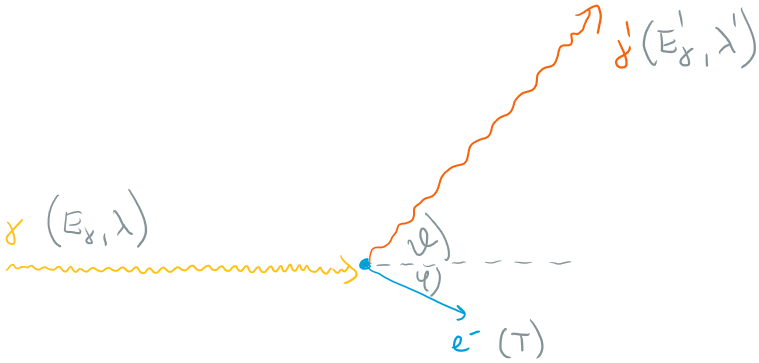
\includegraphics[width=0.6\linewidth]{Compton.png}
            \caption{Comptonův rozptyl fotonu $\gamma$ na elektronu $e^{-}$.}
            \label{fig:Compton}
        \end{figure}

    \subsection{Comptonova vlnová délka}
        Vyjádřete vztah pro změnu vlnové délky fotonu při Comptonově rozptylu $\Delta\lambda=\lambda'-\lambda$ pomocí Comptonovy vlnové délky $\lambda_{c}=h/(m_{e}c)$, kde $h$ je Planckova konstanta, $m_{e}$ hmotnost elektronu a $c$ rychlost světla.

    \subsection{Úhel vylétávajícího elektronu}
        Odvoďte vztah pro úhel $\varphi$, pod kterým vylétá elektron po Comptonově rozptylu (obrázek~\ref{fig:Compton}).

    \subsection{Spektrum $\gamma$ při měření v detektoru}
        \begin{figure}[!h]
            \centering
            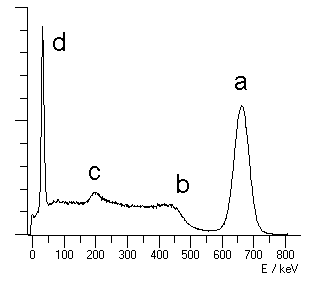
\includegraphics[width=0.35\linewidth]{ComptonSpectrum.png}
            \caption{Detekované Comptonovské spektrum monochromatického $\gamma$ záření.}
            \label{fig:ComptonSpectrum}
        \end{figure}        
    
        Detektor vysokoenergetických kvant $\gamma$ funguje na principu Comptonova rozptylu, kdy kinetická energie rozptýlených elektronů vytvoří impuls elektrického proudu, který se následně zesílí a změří.

        Předpokládejte, že na detektor dopadá monochromatické záření s energií kvant $E_{\gamma}$ vzniklé rozpadem radioaktivního nuklidu.
        Vysvětlete body a, b, c z obrázku~\ref{fig:ComptonSpectrum}; obrázek zobrazuje četnost, se kterou byla detektorem naměřena energie elektronu $E$. 
        Odhadněte, jaká byla energie $E_{\gamma}$, a z této \href{https://cds.cern.ch/record/1309915/files/978-3-642-02586-0_BookBackMatter.pdf}{tabulky} určete nuklid, jehož rozpad je měřen.

        % Zdroj tabulky: https://www.ld-didactic.de/software/524221en/Content/Appendix/ComptonSpectrum.htm\np
\section{Práh reakce}
\subsection{Greisenův-Zatsepinův-Kuzminův limit}
    GZK limit je prahová hodnota energie kosmického protonového záření, nad kterou dojde k interakci protonu s fotonem reliktního záření za vzniku buď protonu a neutrálního pionu, nebo neutronu a kladně nabitého pionu,\footnote{
        K reakci dochází přes $\Delta^{+}$ rezonanci.
    }
    \begin{subequations}
        \begin{align}
            p^{+}+\gamma_{\mathrm{RZ}}
                &\longrightarrow p^{+}+\pi^{0},\\
                &\longrightarrow n^{0}+\pi^{+},
        \end{align}        
    \end{subequations}
    čímž vysokonenergetický foton ztratí energii (je zbržděn).
    Odbvoďte tento limit pro obě reakce.
\np
\section{Rozptyl}
\subsection{Srážkový parametr a diferenciální účinný průřez}
    Odvoďte vztah mezi srážkovým parametrem $b(\theta)$ a diferenciálním účinným průřezem $\derivative{\sigma}{\Omega}$.

\subsection{Rutherfordův rozptyl}
    Vztah pro srážkový parametr u Rutherfordova rozptylu (rozptyl $\alpha$ částice na jádru s protonovým číslem $Z$) na úhel $\theta$ je
    \begin{equation}
        b(\theta)=\frac{d_{0}}{2}\frac{1}{\tg{\frac{\theta}{2}}},
    \end{equation}
    kde
    \begin{equation}
        d_{0}=\frac{2Ze^{2}}{4\pi\epsilon_{0}}\frac{1}{T}
    \end{equation}
    je~\emph{Sommerfeldův parametr} (vzdálenost nejbližšího přiblížení rozptylující a rozptylované částice) a $T$ je kinetická energie $\alpha$ částice v laboratorní soustavě.

    Odvoďte výraz pro diferenciální účinný průřez.

\subsection{Rozptyl na tvrdé kouli}
    \begin{enumerate}
        \item Odvoďte vztah mezi srážkovým parametrem a rozptylem na úhel $\theta$ pro tvrdou kouli.
        \item Odvoďte výraz pro diferenciální účinný průřez.
        \item Určete celkový účinný průřez.
    \end{enumerate}\np
\section{Atom vodíku}
\subsection{Nestabilita klasického atomu}
    Nabitá částice s nábojem $q$ pohybující se se zrychlením $a$ vyzařuje podle klasické teorie elektromagnetického záření s výkonem
    \begin{equation}
        P=\frac{2}{3}\frac{q^2}{4\pi\epsilon}\frac{1}{c^3}a^{2},
    \end{equation}
    kde $\epsilon$ je permitivita a $c$ je rychlost světla.
    Spočítejte, za jak dlouho by dopadl elektron atomu vodíku na jádro, kdyby se pohyboval jako klasická nabitá částice z kruhové dráhy o poloměru daném Bohrovým poloměrem.

    Určete průměrný vyzařovaný výkon.

\subsection{Bohrův model atomu}
    Odvoďte možné hodnoty energií elektronu atomu vodíku za Bohrova předpokladu, že elektron obíhá okolo atomového jádra a že pokud jeho moment hybnosti nabývá celočíselných násobků redukované Planckovy konstanty $\hbar$, nedochází ke zrátě energie Larmorovým vyzařováním.

    Jak se změní výsledek, pokud bude mít jádro náboj $Ze$, $Z>1$?

\subsection{Vlnové délky spektrálních čar atomu vodíku}
    Odvoďte nejkratší a nejdelší vlnovou délku pro Lymanovu, Balmerovu a Paschenovu sérii spektrálních čar atomu vodíku. Které z těchto čar budou ležet ve viditelném světle?

\subsection{Energie fotonů viditelného světla}
    Určete rozmezí energií fotonů viditelného světla.

\subsection{Makroskopický atom}
    Pro jak velké hlavní kvantové číslo bude mít atom vodíku rozměr $r=1\unit{cm}$?

\subsection{Degenerace hladin atomu vodíku}
    Určete stupeň degenerace (počet různých kombinací kvantových čísel, kterými lze získat danou energetickou hladinu) hladiny atomu vodíku s hlavním kvantovým číslem $n$.

\subsection{Poloměr atomu vodíku}
    Ze znalosti radiální části vlnové funkce základního stavu atomu vodíku určete střední poloměr atomu.

\subsection{Mnohaelektronový atom}
    Na základě jednoduchého Bohrova modelu atomu odhadněte rozměr atomu s protonovým číslem~$Z$.

    \begin{enumerate}
    \item
        Jaký je poloměr kruhové dráhy elektronu v Bohrově modelu, pokud jádro nese náboj $Ze$ a hladina má kvantové číslo $n$?
        Vyjádřete v násobcích Bohrova poloměru $a_{0}$ pro atom vodíku.

    \item
        Předpokládejte, atomové jádro s nábojem $Ze$ doplníte $Z$ elektrony, které mezi sebou navzájem neinteragují, a zanedbejte i spin-orbitální vazbu a další případné interakce.
        Jaký bude poloměr výsledného atomu v případě, že je ve valenční slupce jen jeden elektron, a v případě, že je valenční slupka zcela zaplněna?
        Budou atomy větší, nebo menší v porovnání s atomem vodíku?
    \end{enumerate}

    K výpočtu použijte vzorec
    \begin{equation}
        \sum_{n=1}^{N}n^{2}=\frac{N}{6}(N+1)(2N+1).
    \end{equation}\np
\section{Víceelektronové atomy}
\subsection{Unsöldův teorém}
    Dokažte Unsöldův teorém, který říká, že pro dané orbitální kvantové číslo $l$ je součet hustot pravděpodobnosti pro všechny stavy s magnetickým kvantovým číslem $m_l=-l,\dotsc,l$ nezávislý na úhlech $\theta,\phi$.
    Teorém dokažte pro $l=0$, $l=1$, $l=2$.

\subsection{Mnohaelektronový atom}
    Na základě Bohrova modelu atomu odhadněte rozměr atomu s protonovým číslem~$Z$.

    \begin{enumerate}
        \item
            Jaký je poloměr kruhové dráhy elektronu v Bohrově modelu, pokud jádro nese náboj $Ze$ a hladina má kvantové číslo $n$?
            Vyjádřete v násobcích Bohrova poloměru $a_{0}$ pro atom vodíku.

        \item
            Spočítejte poloměr atomu vzácných plynů (zaplněná valenční slupka) a alkalických kovů (jeden elektron ve valenční slupce) a porovnejte s Bohrovým poloměrem $a_{0}$.
    \end{enumerate}

\np
\section{Molekuly a chemická vazba}
    \subsection{Výhřevnost uhlí odhadem}
        Odhadněte výhřevnost uhlí na základě hrubého odhadu, že při reakci hoření uhlí
        \begin{equation}
            \ce{C + O2 -> CO2}
        \end{equation}
        se vznikem jedné molekuly uvolní energie $4\unit{eV}$.
        Kolik váží oxid uhličitý vzniklý spálením $1\unit{kg}$ uhlí?

    \subsection{Výhřevnost uhlí přesně}
        Spočítejte výhřevnost uhlí přesně, pokud znáte slučovací enthalpii
        \begin{equation}
            \Delta H_{f}^{\Theta}(\ce{CO2})=-393\unit{kJ}\unit{mol^{-1}}.
        \end{equation}
        O kolik je důsledkem relativistického vztahu mezi hmotností a energií vzniklý oxid uhličitý lehčí, než jsou hmotnosti konstituentů před reakcí?

    \subsection{Hustoty látek}
        Odhadněte rozmezí hustot kapalin a pevných látek.

    \subsection{Odhadněte výšku hor}
        Předpokládejte, že hory jsou tvořeny křemenem (oxidem křemičitým \ce{SiO2}).
        Odhadněte maximální výšku hor na Zemi a na Marsu.\footnote{Úloha je inspirována článkem~\cite{Weisskopf1975}.}
        Odhadněte, jaká je minimální velikost vesmírného objektu, aby se začal zakulacovat.\np
\section{Nerozlišitelné částice}
    \subsection{Kvantový tlak}
        Určete střední energii jedné částice nerelativistického fermionového plynu o hustotě počtu částic $\rho$.
        Určete, jaký je v tomto plynu tlak.

    \subsection{Relativistický kvantový tlak}
        Zopakujte řešení předchozí úlohy pro ultrarelativistický fermionový plyn (rychlosti částic plynu jsou tak velké, že lze zanedbat jejich klidovou hmotnost).

    \subsection{Poloměr hvězdy}
        Odhadněte poloměr vyhořelé hvězdy (bílého trpaslíka) s hmotností $M$.
        Předpokládejte, že hvězda je složena z uhlíků $^{12}$C.

    \subsection{Chandrasekharova mez}
        Odhadněte Chandrasekharovu mez pro bílého trpaslíka (jedná se o mezní hmotnost, nad kterou již kvantový tlak neudrží hvězdu proti gravitační síle a hvězda se zhroutí do neutronové hvězdy nebo černé díry).

    \subsection{Interakce způsobená nerozlišitelností volných částic}
        Uvažujte dvě nerozlišitelné volné částice o hmotnosti $m$ pohybující se na přímce.
        Jejich vlnové funkce jsou dány gaussovskými balíky dobře lokalizovanými okolo bodů $-b$ a $+b$ (obrázek),
        \begin{equation}
            \psi_{\pm}(x)=\frac{1}{\sqrt[4]{\pi\sigma^{2}}}\e^{-\frac{1}{2\sigma^{2}}(x\mp b)^{2}},
        \end{equation}
        kde $\sigma\ll b$ určuje určuje šířku balíku.
        
        \begin{figure}[htbp!]
            \centering
            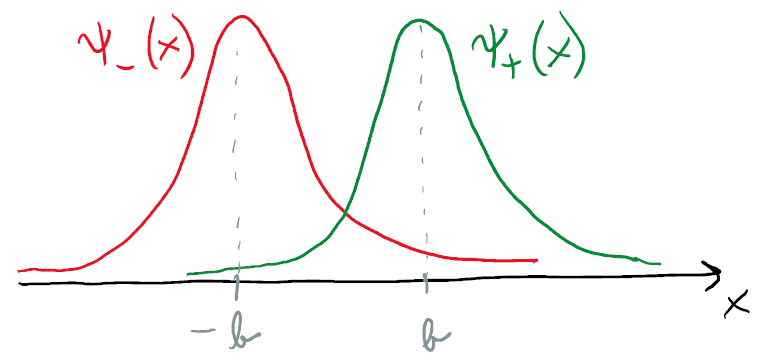
\includegraphics[width=0.5\linewidth]{Identical.png}
        \end{figure}

        \begin{enumerate}
            \item 
                Určete vlnovou funkci $\psi(x_{1},x_{2})$ systému těchto dvou nerozlišitelných částic a spočítejte její normalizaci.
                Vlnové funkce mohou být symetrické (bosony, fermiony s antisymetrickým spinovým stavem) nebo antisymetrické (fermiony se symetrickým spinovým stavem). 
                Uvažujte oba dva případy.
            
            \item Spočítejte střední hodnotu energie systému dvou nerozlišitelných částic
                \begin{equation}
                    E=\matrixelement{\psi}{\operator{H}}{\psi}=\int\psi^{*}(x_{1},x_{2})H\psi(x_{1},x_{2})\d x_{1}\d x_{2}.
                \end{equation}

            \item Spočítejte efektivní sílu
                \begin{equation}
                    F\equiv-\frac{\partial E}{\partial b}.
                \end{equation}
                Bude tato síla přitažlivá nebo odpudivá a jak závisí na symetrii vlnové funkce?
        \end{enumerate}
\np
\section{Kvantové provázání}
    \subsection{Kvantová teleportace}
        Popište, jakým způsobem lze přenést stav kvantového qubitu z místa A do místa B pomocí klasického komunikačního kanálu. Tento jev se nazývá kvantová teleportace.

    \subsection{Provázaný stav}
        Dokažte, že provázaný stav dvou qubitů 
        \begin{equation}
            \ket{\Psi}=\frac{1}{\sqrt{2}}\left(\ket{\uparrow}_{1}\ket{\uparrow}_{2}+\ket{\downarrow}_{1}\ket{\downarrow}_{2}\right)
        \end{equation}
        nelze faktorizovat, tj. nelze ho napsat ve tvaru
        \begin{equation}
            \left(\alpha\ket{\uparrow}+\beta\ket{\downarrow}\right)_{1}\left(\gamma\ket{\uparrow}+\delta\ket{\downarrow}\right)_{2},\quad\alpha,\beta,\gamma,\delta\in\mathbb{C}.
        \end{equation}

    \subsection{Stav dvouqubitového systému}
        Rozhodněte, zda stav dvou qubitů
        \begin{equation}
    \ket{\Phi}=\mathcal{N}\left(2\ket{\uparrow\uparrow}+\im\ket{\downarrow\uparrow}+4\im\ket{\uparrow\downarrow}-2\ket{\downarrow\downarrow}\right)
        \end{equation}
        je provázaný, a svou odpověď zdůvodněte. 
        Nalezněte normalizační faktor $\mathcal{N}$.

        V zápisu stavu je použito zjednodušeného značení $\ket{\uparrow\downarrow}\equiv\ket{\uparrow}_{1}\otimes\ket{\downarrow}_{2}$ (analogicky i pro ostatní kombinace spinu nahoru a dolů).
\np
\section{Užitečné vztahy}

\subsection{Vzorce}
\begin{itemize}
    \item Planckův vyzařovací zákon ve frekvencích $\nu$
        \begin{equation}
            \rho(\nu,T)\d\nu=\frac{8\pi h}{c^{3}}\frac{1}{\e^{\frac{h\nu}{k_{B}T}}-1}\nu^{3}\d\nu
        \end{equation}

    \item Planckův vyzařovací zákon ve vlnových délkách $\lambda$
        \begin{equation}
            \rho(\lambda,T)\d\lambda=8\pi h c\frac{1}{\e^{\frac{h c}{\lambda k_{B}T}}-1}\frac{\d\lambda}{\lambda^{5}}
        \end{equation}

    \item Wienův posunovací zákon
        \begin{align}
            \lambda_{\mathrm{max}}&=\frac{\alpha}{T}&\alpha&\approx 2\c90\cdot10^{-3}\unit{mK}\\
            \nu_{\mathrm{max}}&=\beta\,T & \beta&\approx 5\c83\cdot 10^{10}\unit{K^{-1}s^{-1}}
        \end{align}

    \item Stefanův-Boltzmannův zákon
        \begin{align}
            M&=\sigma T^{4} & \sigma&=\frac{2\pi^{5}k_{B}^{4}}{15h^{3}c^{2}}\approx 5\c67\cdot10^{-8}\unit{Wm^{-2}K^{-4}}
        \end{align}

    \item Vztah mezi energií $E$, vlnovou délkou $\lambda$ a frekvencí $\nu$ kvant elektromagnetického záření
        \begin{equation}
            E=h\nu=\frac{hc}{\lambda}
        \end{equation}

    \item Comptonův rozptyl
        \begin{align}
            \lambda'-\lambda&=\lambda_{c}\left(1-\cos\theta\right) & \lambda_{c}&=\frac{h}{m_{e}c}
        \end{align}

    \item Rutherfordův rozptyl částice s nábojem $ze$ a kinetickou energií $T$ na jádře s nábojem $Ze$
        \begin{align}
            b&=\frac{d_{0}}{2}\frac{1}{\tg{\frac{\theta}{2}}} & d_{0}&=\frac{Zze^{2}}{4\pi\epsilon_{0}}\frac{1}{T}\\
            \derivative{\sigma}{\theta}&=\left(\frac{d_{0}}{4}\right)^{2}\frac{1}{\sin^{4}{\frac{\theta}{2}}}
        \end{align}

    \item Spektrum vodíkupodobného atomu s centrálním nábojem $Ze$ a obíhající částicí hmotnosti $m$
        \begin{equation}
            E_{n}=R_{\infty}\frac{m}{m_{e}}Z^{2}\frac{1}{n^{2}}
        \end{equation}

    \item Relativistický vztah mezi energií $E$ a hybností $p$
        \begin{equation}
            E^{2}=\left(Mc^{2}\right)^{2}=\left(M_{0}c^{2}\right)^{2}+\left(pc\right)^{2}
        \end{equation}

\end{itemize}

\subsection{Konstanty}
\begin{itemize}
    \item Planckova konstanta
        \begin{align}
            h&\approx6\c63\cdot 10^{-34}\unit{Js}\\
            \hbar&\equiv\frac{h}{2\pi}\approx1\c05\cdot 10^{-34}\unit{Js}.
        \end{align}

    \item Rychlost světla ve vakuu
        \begin{equation}
            c\approx 3\c00\cdot 10^{8}\unit{ms^{-1}}
        \end{equation}
    
    \item Hmotnost elektronu
        \begin{equation}
            m_{e}\approx 9.11\cdot 10^{-31}\unit{kg}\approx 511\unit{keV}
        \end{equation}

    \item Elementární náboj
        \begin{equation}
            e\approx 1.60\cdot 10^{-19}\unit{C}
        \end{equation}

    \item Konstanta jemné struktury
        \begin{equation}
            \alpha=\frac{e^{2}}{4\pi\epsilon_{0}}\frac{1}{\hbar c}\approx\frac{1}{137}
        \end{equation}

    \item Rydbergova konstanta
        \begin{equation}
            R_{\infty}=\left(\frac{e^{2}}{4\pi\epsilon_{0}}\right)^{2}\frac{m_{e}}{2h^{2}}=hc\frac{\alpha^{2}}{2\lambda_{c}}\approx 13\c6\unit{eV}
        \end{equation}

    \item Comptonova vlnová délka
        \begin{equation}
            \lambda_{c}=\frac{h}{m_{e}c}\approx2\c43\cdot10^{-12}\unit{m}
        \end{equation}

    \item Bohrův poloměr
        \begin{equation}
            a_{0}=\frac{4\pi\epsilon_{0}}{e^{2}}\frac{\hbar^{2}}{m_{e}}=\frac{\lambda_{c}}{\alpha}\approx5\c3\cdot10^{-11}\unit{m}
        \end{equation}

    \item Boltzmannova konstanta
        \begin{equation}
            k_{B}\approx1\c38\cdot10^{-23}\unit{\frac{J}{K}}
        \end{equation}

    \item Termodynamická teplota
        \begin{equation}
            T(0\unit{^{\circ}C})\approx273\c15\unit{K}
        \end{equation}

    \item Avogadrova konstanta
        \begin{equation}
            N_{A}\approx6\c023\cdot10^{23}\unit{mol^{-1}}
        \end{equation}
\end{itemize}

\subsection{Jednoelektronový atom}
\begin{itemize}
    \item Radiální vlnové funkce ($Z$ je náboj jádra v jednotkách $e$)
        \begin{align}
            R_{10}(r)&=2\left(\frac{Z}{a_{0}}\right)^{\frac{3}{2}}\e^{-\frac{Zr}{a_{0}}}\\
            R_{20}(r)&=2\left(\frac{Z}{2a_{0}}\right)^{\frac{3}{2}}\left(1-\frac{Zr}{2a_{0}}\right)\e^{-\frac{Zr}{2a_{0}}}\\
            R_{21}(r)&=\frac{1}{\sqrt{3}}\left(\frac{Z}{2a_{0}}\right)^{\frac{3}{2}}\left(\frac{Zr}{a_{0}}\right)\e^{-\frac{Zr}{2a_{0}}}\\
            R_{30}(r)&=2\left(\frac{Z}{3a_{0}}\right)^{\frac{3}{2}}\left(1-\frac{2Zr}{3a_{0}}+\frac{2Z^{2}r^{2}}{27a_{0}^{2}}\right)\e^{-\frac{Zr}{3a_{0}}}\\
            R_{31}(r)&=\frac{4\sqrt{2}}{3}\left(\frac{Z}{3a_{0}}\right)^{\frac{3}{2}}\left(\frac{Zr}{a_{0}}\right)\left(1-\frac{Zr}{6a_{0}}\right)\e^{-\frac{Zr}{3a_{0}}}\\
            R_{32}(r)&=\frac{2\sqrt{2}}{27\sqrt{5}}\left(\frac{Z}{3a_{0}}\right)^{\frac{3}{2}}\left(\frac{Zr}{a_{0}}\right)^{2}\e^{-\frac{Zr}{3a_{0}}}
        \end{align}
\end{itemize}\np

\begin{homework}
\exercise[15.10.2024]{Fotonová plachetnice}
    Čtvercová plachta o rozměrech $d\times d$ se nachází ve vesmíru ve vzdálenosti $R$ od Slunce.
	\begin{enumerate}
		\item Určete, jaká síla bude na plachtu působit díky slunečnímu záření, víte-li, že zářivý výkon Slunce na povrchu Země je $I_{z}$.
		\item Jak musí být plachta orientovaná, aby byla síla od záření co největší?
		\item Je síla větší, když plachta záření pohltí, nebo když ho odrazí?
		\item Zahrňte do výpočtu i gravitační sílu působící na plachtu. 
			Předpokládejte, že plachta je vyrobena z hliníku (alobalu) o hustotě $\rho$.
			Jakou musí mít tloušťku, aby tlak záření překonal gravitační sílu?
	\end{enumerate}
	Řešte nejprve obecně, pak pro číselné hodnoty $\rho=2700\unit{kg\,m^{-3}}$, $d=100\unit{m}$, $I_z=1370\unit{W/m^{2}}$.
	Využijte vztahu mezi energií a hybností fotonů $E=pc$.    
\end{homework}

\begin{homework}
\exercise[29.10.2024]{Elektron při Comptonově rozptylu}
	\begin{itemize}
	\item
		Odvoďte vztah pro úhel $\varphi$, pod kterým vylétá elektron $e^{-}$ po Comptonově rozptylu, a vyjádřete ho pomocí vlnových délek nalétávajícího a rozptýleného fotonu $\lambda,\lambda'$ a Comptonovy vlnové délky $\lambda_{C}=h/(m_{e}c)$.
		\begin{center}
			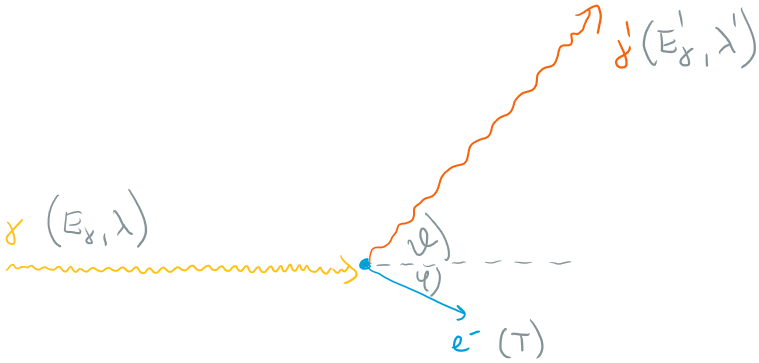
\includegraphics[width=0.8\linewidth]{Compton.png}
		\end{center}
	
	\item 
		Zakreslete graf závislosti $\varphi(\lambda')$ pro $\lambda'\in(\lambda,\lambda+2\lambda_{C})$ a vhodně zvolené $\lambda$.

	\end{itemize}
	\emph{Nápověda:} Vyjděte ze zákona zachování hybnosti ve směru nalétávajícího fotonu $\gamma$ a ve směru kolmém.
\end{homework}

\begin{homework}
	\exercise[26.11.2024]{Klasický model atomu vodíku}
	\begin{itemize}
		\item     
			Nalezněte vztah pro frekvenci kruhového pohybu elektronu v klasickém modelu vodíkového atomu za předpokladu, že elektron neztrácí energii vyzařováním a že se nachází ve vzdálenosti $r=\beta a_{0}$ od protonu, kde $a_{0}$ je Bohrův poloměr.
			Výsledný vztah {\bf vyjádřete pomocí konstanty jemné struktury $\alpha$}.
			Vypočítejte číselně pro $\beta=1$.

		\item
			Jaká bude velikost $\beta$, pokud elektron obíhá proton se zadanou frekvencí $f$?
			Jaké hodnotě kvantového čísla $n$ Bohrova modelu atomu vodíku by odpovídala tato oběžná dráha?
			Vyřešte obecně a pak pro číselnou hodnotu $f=1\unit{Hz}$.

		\item
			Na cvičení jsme si ukázali, že obíhající elektron ve skutečnosti kvůli dostředivému zrychlení postupně ztrácí energii elektromagnetickým vyzařováním, a odvodili jsme vztah pro dobu $T$, za kterou elektron v atomu vodíku \uv{spadne} na proton.
			Nalezněte vztah pro okamžitý vyzařovaný výkon v čase $P(t)$ a vykreslete graf pro $t\in[0,T]$.
			Elektron je v čase $t=0$ na orbitě s poloměrem $a_{0}$.
	\end{itemize}
\end{homework}

\begin{homework}
	\exercise[10.12.2024]{Rozměr vzbuzeného vodíku}
		Vodík se nachází ve vzbuzeném $2s$ stavu.
		Jeho radiální část vlnové funkce je tedy
		\begin{equation*}
			R_{20}(r)=2\left(\frac{1}{2a_{0}}\right)^{\frac{3}{2}}\left(1-\frac{r}{2a_{0}}\right)\e^{-\frac{r}{2a_0}}.
		\end{equation*}

		\begin{enumerate}
			\item
				Nalezněte vzdálenost $r_{p}$ od jádra, na které naměříte elektron s největší pravděpodobností.

			\item
				Určete střední poloměr atomu (střední hodnotu vzdálenost $\langle r\rangle$ od jádra, na které naměříte elektron).

			\item
				Jak se změní měřený rozměr atomu, pokud se vodík bude nacházet ve $2p$ stavu, jehož radiální část vlnové funkce je
				\begin{equation*}
					R_{21}(r)=\frac{1}{\sqrt{3}}\left(\frac{1}{2a_{0}}\right)^{\frac{3}{2}}\frac{r}{a_{0}}\e^{-\frac{r}{2a_{0}}}?
				\end{equation*}

			\item
				Jaká bude vlnová délka vyzářeného fotonu, když elektron spadne ze vzbuzeného stavu do základního stavu?
				Bude možné tento přechod pozorovat pouhým okem?

			\item
				Vyhledejte si vyjádření kulových funkcí pro $p$ podslupku a dokažte, že pro ni platí Unsöldův teorém (tj. že tato uzavřená podslupka má sféricky symetrické rozložení náboje).
		\end{enumerate}

		\newpage
\end{homework}

% \begin{homework}
% \exercise[9.10.2023]{Žárovka}
% 	\begin{enumerate}
% 		\item
% 			Odhadněte délku a poloměr wolframového vlákna žárovky s příkonem $P=100\unit{W}$ zapojené v~české elektrické síti, víte-li, že teplota svítícího vlákna je $T=2700\unit{K}$ a měrný elektrický odpor wolframu při teplotě $t=20\unit{^{o}C}$ je $\rho_{0}=5\c6\cdot10^{-8}\,\Omega\unit{m}$.
% 			Předpokládejte, že odpor vlákna závisí lineárně na teplotě,
% 			\begin{equation*}
% 				R=R_{0}(1+\alpha\Delta t),
% 			\end{equation*}
% 			kde $\alpha=4\c5\cdot10^{-3}\unit{K^{-1}}$ je teplotní součinitel elektrického odporu pro wolfram a $\Delta t$ je rozdíl teplot.

% 		\item
% 		    Jaké procento energie vyzařované vláknem je ve viditelné části spektra mezi vlnovými délkami $\lambda\in[380\unit{nm},750\unit{nm}]$?
% 			Kam se \uv{ztratí} zbývající část vyzařované energie?
% 	\end{enumerate}

% 	\newpage
% \end{homework}
	
% \begin{homework}
% 	\setcounter{figure}{0}
% 	\pagestyle{empty}
% 	\exercise[23.10.2023]{Polovodičový detektor $\gamma$ záření}
% 	K detekci ionizujícího záření se používají polovodičové detektory.
% 	Budeme předpokládat, že na detektor dopadá monochromatické záření s energií kvant $E_{\gamma}$ vzniklé rozpadem radioaktivního nuklidu.
% 	Vysokoenergetické fotony interagují s elektrony polovodičového krystalu a předávají jim kinetickou energii $T$, což vytváří v detektoru elektrické impulsy, který se následně zesílí a změří.
% 	Výsledkem měření je graf zobrazený na obrázku~\ref{fig:ComptonSpectrum}, kde na vodorovné ose je kinetická energie $T$ rozptýlených elektronů a na svislé ose četnost, se kterou byla tato energie naměřena při velkém počtu opakování měření.

% 	\begin{figure}[!h]
% 		\centering
% 		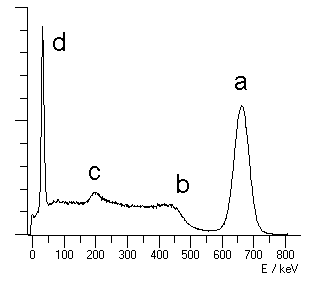
\includegraphics[width=0.5\linewidth]{ComptonSpectrum.png}
% 		\caption{Detekované spektrum monochromatického $\gamma$ záření polovodičovým detektorem.}
% 		\label{fig:ComptonSpectrum}
% 	\end{figure}        

% 	\begin{figure}[!h]
% 		\centering
% 		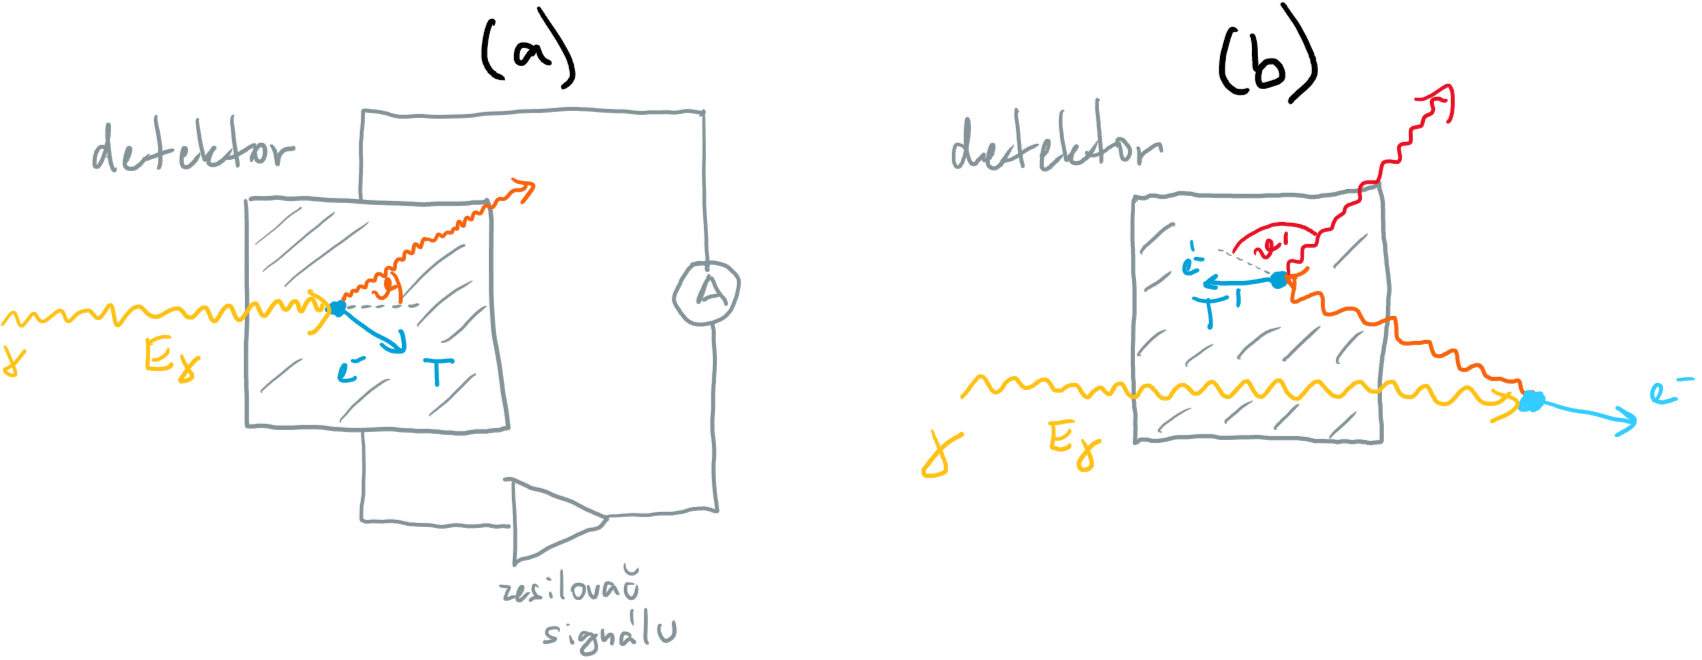
\includegraphics[width=0.9\linewidth]{ComptonDetector.png}
% 		\caption{Comptonův rozptyl. (a) Uvnitř detektoru. (b) Primární rozptyl vně detektoru, sekundární rozptyl uvnitř detektoru.}
% 		\label{fig:ComptonDetector}
% 	\end{figure}        

% 	Jeden z procesů je Comptonův rozptyl, schematicky znázorněný na obrázku~\ref{fig:ComptonSpectrum}.	
% 	\begin{enumerate}
% 		\item Určete rozmezí energií $(T_{\mathrm{min}},T_{\mathrm{max}})$, které lze očekávat při Comptonově rozptylu fotonů s energií $E_{\gamma}$ uvnitř detektoru, přičemž rozptýlený foton vylétne z detektoru ven.
% 		Proces je zobrazen na obrázku~\ref{fig:ComptonDetector}~(a).
% 		Energie $T_{\mathrm{max}}$ ve změřeném spektru udává tzv. \emph{Comptonovu hranu}.

% 		\item Ke Comptonově rozptylu fotonů může dojít i mimo detektor, což je znázorněno na obrázku~\ref{fig:ComptonDetector}~(b).
% 		Do detektoru pak vlétají fotony s nižší energií.
% 		Předpokládejte, že fotony rozptýlené o libovolný úhel vně detektoru se následně v detektoru rozptýlí vždy o úhel $\vartheta'=180^{\mathrm{o}}$ (pravděpodobnost zpětného rozptylu je vždy nejvyšší podle tzv. Kleinova-Nishinova zákona).
% 		Určete, jaké rozmezí detekovaných energií $(T'_{\mathrm{min}},T'_{\mathrm{max}})$ lze očekávat v tomto případě.
% 		Energie $T'_{\mathrm{min}}$ ve změřeném spektru udává tzv. \emph{pík zpětného odrazu}.

% 		\item Identifikujte v obrázku~\ref{fig:ComptonSpectrum} Comptonovu hranu i pík zpětného odrazu a spočítejte z nich energii $E_{\gamma}$ nalétávajících fotonů.
% 		Z tabulky na adrese \url{https://cds.cern.ch/record/1309915/files/978-3-642-02586-0_BookBackMatter.pdf} určete nuklid, jehož rozpad je měřen.

% 		\item
% 			Kromě Comptonova rozptylu dochází také k fotoefektu, při kterém je nalétávající foton zcela pohlcen.
% 			Identifikujte v obrázku~\ref{fig:ComptonSpectrum} pík odpovídající fotoefektu a určete z něj energii detekovaných fotonů $E_{\gamma}$.
% 			Předpokládejte, že ionizační energie elektronů je zanedbatelná vůči~$E_{\gamma}$.

% 		\item
% 		Při dostatečně vysoké energii záření $E_{\gamma}$ dochází v detektoru i ke vzniku elektron-pozitronového páru. Může k tomu jevu docházet i v případě měření z obrázku~\ref{fig:ComptonSpectrum}?
% 	\end{enumerate}

% 	\newpage
% \end{homework}

% \begin{homework}
% 	\exercise[30.10.2023]{Rutherfordův rozptyl}
%     Protony vylétávají z urychlovače s kinetickou energií $T=200\,\mathrm{MeV}$, dopadají na velmi tenkou hliníkovou fólii o tloušťce $t=100\unit{nm}$ a dochází k rozptylu.
%     Svazek má tok $\Phi=10^{9}$ protonů za sekundu.
% 	Hustota hliníku je $\rho=2710\unit{kg}\unit{m^{-3}}$.

%     \begin{itemize}
%         \item Určete diferenciální účinný průřez Rutherfordova rozptylu protonů na úhel $\theta=30^{\mathrm{o}}$.
%         \item Spočítejte celkový účinný průřez na úhly větší než $\theta_0=90^{\mathrm{o}}$.
%         \item Vyjádřete tloušťku fólie v počtu atomů hliníku.
%         \item Kolik protonů za sekundu se rozptýlí na úhly větší než $\theta_0$?
%     \end{itemize}

% \newpage
% \end{homework}
	
% \begin{homework}
% 	\exercise[6.11.2023]{Klasický model vodíku}
% 	\begin{itemize}
% 		\item     
% 			Spočítejte frekvenci kruhového pohybu elektronu v klasickém modelu vodíkového atomu (elektron se nachází ve vzdálenosti Bohrova poloměru $a_{0}$ od atomového jádra).
% 			Výsledný vztah vyjádřete pomocí konstanty jemné struktury $\alpha$.
% 		\item
% 			Pokud by elektron vyzařoval elektromagnetické záření o této frekvenci, jaké by mělo vlnovou délku a v jaké oblasti spektra by se nacházelo?
% 		\item
% 			Jak daleko od protonu by elektron musel být, aby obíhal s frekvencí $f=1\unit{s^{-1}}$?
% 	\end{itemize}

% \newpage
% \end{homework}

% \begin{homework}
% 	\exercise{Rozměr vzbuzeného vodíku}
% 		Vodík se nachází ve vzbuzeném $2s$ stavu.
% 		Jeho radiální část vlnové funkce je tedy
% 		\begin{equation*}
% 			R_{20}(r)=2\left(\frac{1}{2a_{0}}\right)^{\frac{3}{2}}\left(1-\frac{r}{2a_{0}}\right)\e^{-\frac{r}{2a_0}}.
% 		\end{equation*}

% 		\begin{enumerate}
% 			\item
% 				Nalezněte vzdálenost $r_{p}$ od jádra, na které naměříte elektron s největší pravděpodobností.
% 			\item
% 				Určete střední poloměr atomu (střední hodnotu vzdálenost $\langle r\rangle$ od jádra, na které naměříte elektron).
% 			\item
% 				Jak se změní měřený rozměr atomu, pokud se vodík bude nacházet ve $2p$ stavu, jehož radiální část vlnové funkce zní
% 				\begin{equation*}
% 					R_{21}(r)=\frac{1}{\sqrt{3}}\left(\frac{1}{2a_{0}}\right)^{\frac{3}{2}}\frac{r}{a_{0}}\e^{-\frac{r}{2a_{0}}}?
% 				\end{equation*}
% 			\item
% 				Jaká bude vlnová délka vyzářeného fotonu, když elektron spadne do základního stavu?
% 				Bude možné tento přechod pozorovat pouhým okem?
% 		\end{enumerate}

% 		\newpage
% \end{homework}

% \begin{homework}
% 	\exercise{Pálení uhlí}
% 		Černé uhlí je tvořeno z převážné části uhlíkem. Spálením $M=1\unit{kg}$ uhlíku se uvolní $Q=33\unit{MJ}$ energie ve formě tepla.
% 		\begin{enumerate}
% 			\item 
% 				Jaká hmotnost oxidu uhličitého $\ce{CO2}$ vznikne spálením $M=1\unit{kg}$ uhlíku, tj. při reakci
% 				\begin{equation*}
% 					\ce{C + O2 -> CO2}?
% 				\end{equation*}

% 			\item
% 				Kolik litrů vody ohřejete z pokojové teploty na teplotu varu spálením $M=1\unit{kg}$ uhlíku za předpokladu, že se veškerá energie vzniklá hořením uhlíku využije na ohřev vody?

% 			\item
% 				Důsledkem relativistické relace mezi energií a hmotností $E=mc^{2}$, kde $c$ je rychlost světla, se bude hmotnost vzniklého $\ce{CO2}$ lišit od hmotnosti reaktantů $\ce{C}$ a $\ce{O2}$.
% 				Jak velký bude tento rozdíl?

% 				Tepelná elektrárna spálí $10$ tun uhlí za minutu.
% 				Kolik let musí elektrárna běžet, aby byl tento relativistický rozdíl $m=1\unit{kg}$?
% 				Předpokládejte, že pálené uhlí je tvořeno pouze uhlíkem.
% 		\end{enumerate}

% 		\newpage
% \end{homework}

% \begin{homework}
% 	\exercise{Zhroucení Slunce}
% 		Předpokládejte, že naše Slunce se po vyhoření zhroutí a vznikne z něj bílý trpaslík tvořený pouze uhlíkem $^{12}\mathrm{C}$.  
% 		Předpokládejte, že hustota trpaslíka je konstantní.

% 		\begin{enumerate}
% 			\item Spočítejte Fermiho energii $E_{F}$ nerelativistického elektronového degenerovaného plynu a Fermiho rychlost $v_{F}$ danou vztahem
% 			\begin{equation*}
% 				E_{F}=\frac{1}{2}m_{e}v_{F}^{2}.
% 			\end{equation*}
% 			Vyjádřete Fermiho rychlost v násobcích rychlosti světla.
% 			Je nerelativistická aproximace oprávněná?
			
% 			\item Na základě uvedených předpokladů určete poloměr vzniklého bílého trpaslíka.

% 			\item Předpokládejte, že degenerovaný elektronový plyn je ultrarelativistický a určete Chandrasekharovu mez.
% 				Najděte její číselnou hodnotu vyjádřenou v násobcích hmotnosti Slunce.
			
% 			\item Je-li hvězda těžší, než kolik udává Chandrasekharova mez, dojde k jejímu dalšímu zhroucení a vznikne neutronová hvězda.
% 			Spočítejte mezní hmotnost pro sférickou hvězdu o konstantní hustotě tvořenou degenerovaným neutronovým plynem (nazývá se Tolmanova-Oppenheimerova-Volkoffova mez) a vyjádřete ji v násobcích hmotnosti Slunce.
% 		\end{enumerate}

% 		{\it Poznámka:} Předpoklad konstantní hustoty je velmi hrubý. 
% 		Po započtení hustoty správně rostoucí s hloubkou pod povrchem a dalších korekcí vycházejí obě meze nižší.

% 		\newpage
% \end{homework}

% \begin{homework}
% 	\exercise{Kvantové provázání a teleportace}
% 	\begin{enumerate}
% 		\item 
% 		Rozhodněte, zda stav dvou qubitů
% 		\begin{equation*}
% 			\ket{\Phi}=\mathcal{N}\left(2\ket{\uparrow\uparrow}+\im\ket{\downarrow\uparrow}+4\im\ket{\uparrow\downarrow}-2\ket{\downarrow\downarrow}\right)
% 		\end{equation*}
% 		je provázaný, a svou odpověď zdůvodněte. 
% 		Nalezněte normalizační faktor $\mathcal{N}$.

% 		\item
% 		Bude kvantová teleportace qubitu v obecném stavu $\ket{\psi}=\alpha\ket{\uparrow}+\beta\ket{\downarrow}$ od Alice k Bobovi fungovat i v případě, že Alice a Bob budou mít k dispozici provázaný Bellův stav
% 		\begin{equation*}
% 			\ket{\Psi^{+}}=\frac{1}{\sqrt{2}}\left[\ket{\uparrow\downarrow}+\ket{\downarrow\uparrow}\right]?
% 		\end{equation*}
% 		Pokud ano, jako transformaci musí provést Bob na základě klasické informace získané od Alice, aby získal stav identický s tím, který Alice odesílala?
% 	\end{enumerate}

% 	V zápisu stavů je použito zjednodušeného značení $\ket{\uparrow\downarrow}\equiv\ket{\uparrow}_{1}\ket{\downarrow}_{2}$ (analogicky i pro ostatní kombinace spinu nahoru a dolů a pro ostatní kombinace podsystémů).

% 	\newpage
% \end{homework}

\np

\printindex

%\bibliography{Z:/Share/Fyzika/Bibliography/References.bib}
\printbibliography
%\input{refs}

\end{document}
